\section{麦克斯韦方程组}
麦克斯韦电磁理论的基础是本章\xref{sec:真空中静电场的基本规律}、\xref{sec:真空中静磁场的基本规律}、\xref{sec:电磁感应和位移电流}中提到的电磁学三大实验定律:库伦定律、安培力定律、法拉第电磁感应定律。这三个实验定律都是在各自的特定条件下总结出来的,而麦克斯韦在前人得到的实验结果的基础上,通过科学的假设和符合逻辑的分析,最终在1864年,归纳总结出了\uwave{麦克斯韦方程组}(Maxwell's Equations),由此统一了电磁理论。

\begin{Figure}[麦克斯韦]
    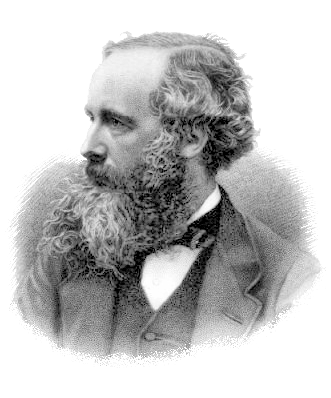
\includegraphics[width=4.4cm]{image/James_Clerk_Maxwell.png}
\end{Figure}

\subsection{麦克斯韦方程组}
麦克斯韦方程组实质上,就是对前面五个小节结论的汇总,它完整的表述了电磁场的性质。\footnote{记得高二那年初次听闻麦克斯韦方程组,那时,虽不知其意,但仍被其优美和简洁所震撼。时至今日,已经过去了整整三年,我想这一天对我来说会是一个值得纪念的日子,三年的等待,三年的准备,我终于看见了电磁波。—— 2023.03.24 写于钱伟长图书馆}
\begin{BoxEquation}[麦克斯韦方程组]
    麦克斯韦方程组描述了电磁场的基本形状,包含以下四个方程
    \begin{Gather}[10pt]
        \curl\vb*{H}=\vb*{J}+\pdv{\vb*{D}}{t}\xlabelpeq{磁场旋度}\\
        \curl\vb*{E}=-\pdv{\vb*{B}}{t}\xlabelpeq{电场旋度}\\
        \div\vb*{B}=0\xlabelpeq{磁场散度}\\
        \div\vb*{D}=\rho\xlabelpeq{电场散度}
    \end{Gather}
    除此之外,另有三组本构关系作为电磁场的辅助方程
    \begin{Equation}
        \vb*{D}=\varepsilon\vb*{E}\qquad
        \vb*{B}=\mu\vb*{H}\qquad
        \vb*{J}=\sigma\vb*{E}
    \end{Equation}
\end{BoxEquation}

麦克斯韦方程组,从内容上看,其实就是阐述了以下四个事实
\begin{center}
    \ttfamily

    电荷是电场的通量源,电流是磁场的涡旋源

    变化的磁场是电场的负涡旋源,变化的电场是磁场的正涡旋源
\end{center}
麦克斯韦的方程组的四个方程,依次从旋度和散度说明了磁场和电场的性质
\begin{enumerate}
    \item 磁场的旋度,源自变化的电场和传导电流。
    \item 电场的旋度,源自变化的磁场。
    \item 磁场的散度,始终为零。
    \item 电场的散度,源自电荷。
\end{enumerate}
我们可能会注意到,尽管麦克斯韦方程组的数学形式非常优美,但是好像总有一些不对称,这种不对称性其实来自,我们只有“电荷和电流”,并没有所谓“磁荷和磁流”,假如磁荷真的存在的话\cite{W3},那么$\div\vb*{B}$即为磁荷,而$\curl\vb*{E}$中亦要补充磁流项,这样方程就完全对应了。\footnote{虽然这样说,但或许正是电场和磁场间,以及千千万万更多事物间的不对称性,才有了我们这个精彩而灵动的世界。}

麦克斯韦方程组亦有积分形式,列写如下
\begin{Gather}[12pt]
    \Ilot[C]\vb*{H}\cdot\dd{\vb*{l}}=\Isnt[S]\qty(\vb*{J}+\pdv{\vb*{D}}{t})\cdot\dd{\vb*{S}}\\
    \Ilot[C]\vb*{E}\cdot\dd{\vb*{l}}=-\Isnt[S]\pdv{\vb*{B}}{t}\cdot\dd{\vb*{S}}\\
    \Isot[S]\vb*{B}\cdot\dd{\vb*{S}}=0\\
    \Isot[S]\vb*{D}\cdot\dd{\vb*{S}}=\Itnt[V]\rho\dd{V}
\end{Gather}
但在实际应用中,我们还是会更多的使用麦克斯韦方程的微分形式而不是积分形式。


实际上,在时变条件下,麦克斯韦方程组的四个方程之间并不是完全独立的,我们可以由它的两个旋度方程部分推导出两个散度方程,至多允许与原有的两个散度方程相差一个常数。\footnote{所以,实际上还是不独立的?或者说,两个散度方程的意义就是明确这个常数的值?}

\paragraph{由电场旋度方程推导磁场散度方程}
我们在电场的旋度方程\xrefpeq{电场旋度}两端取散度
\begin{Equation}
    \div(\curl\vb*{E})=-\pdv{t}(\div\vb*{B})
\end{Equation}
由于旋度的散度为零,这里$\div(\curl\vb*{E})=0$
\begin{Equation}
    \pdv{t}(\div\vb*{B})=0
\end{Equation}
这表明$\div\vb*{B}=$是常数,这与磁场散度方程的$\div\vb*{B}=0$至多相差一个常数。

\paragraph{由磁场旋度方程推导电场散度方程}
我们在磁场的旋度方程\xrefpeq{磁场旋度}两端取散度
\begin{Equation}
    \div(\curl\vb*{H})=\div\vb*{J}+\pdv{t}(\div\vb*{D})
\end{Equation}
由于旋度的散度为零,这里$\div(\curl\vb*{H})=0$
\begin{Equation}
    \pdv{t}(\div\vb*{D})+\div\vb*{J}=0
\end{Equation}
代入\fancyref{eqt:电流连续性方程},即$\div\vb*{J}=-\pdv*{\rho}{t}$
\begin{Equation}
    \pdv{t}(\div\vb*{D}-\rho)=0
\end{Equation}
这表明$\div\vb*{D}-\rho$是常数,这与电场散度方程\xrefpeq{电场散度}的$\div\vb*{D}=\rho$至多相差一个常数。

\subsection{电准静态电磁场}
在麦克斯韦方程组中,若$\pdv*{\vb*{B}}{t}$项可以忽略,即感应电场远小于库伦电场,例如电容器中的电磁场,则可以得到\uwave{电准静态电磁场},电准静态下,尽管$\vb*{E},\vb*{D}$时变,但却适用静电场的规律。
\begin{BoxEquation}[电准静态电磁场]
    电准静态电磁场,是指$\pdv*{\vb*{B}}{t}$项可以忽略,此时麦克斯韦方程组
    \begin{Gather}[10pt]
        \curl\vb*{H}=\vb*{J}+\pdv{\vb*{D}}{t}\\
        \curl\vb*{E}=0\\
        \div\vb*{B}=0\\
        \div\vb*{D}=\rho
    \end{Gather}
\end{BoxEquation}

\subsection{磁准静态电磁场}
在麦克斯韦方程组中,若$\pdv*{\vb*{D}}{t}$项可以忽略,即位移电流远小于传导电流,例如电感器中的电磁场,则可以得到\uwave{磁准静态电磁场},磁准静态下,尽管$\vb*{B},\vb*{H}$时变,但却适用静磁场的规律。
\begin{BoxEquation}[磁准静态电磁场]
    磁准静态电磁场,是指$\pdv*{\vb*{D}}{t}$项可以忽略,此时麦克斯韦方程组
    \begin{Gather}[10pt]
        \curl\vb*{H}=\vb*{J}\\
        \curl\vb*{E}=-\pdv{\vb*{B}}{t}\\
        \div\vb*{B}=0\\
        \div\vb*{D}=\rho
    \end{Gather}
\end{BoxEquation}